% Nome do capítulo
% Diminuir espaçamento entre título e texto


\chapter{Considerações finais}
\label{conslusao-e-trabalhos-furutos}
\vspace{-1.9cm}

  Neste capítulo são apresentadas as considerações finais, as contribuições do
  trabalho e as perspectivas futuras.

% Texto do capítulo
  Conforme a pesquisa do \cite{ibge} número de usuários conectados a Internet tem crescido bastante e é necessário
  que os aplicativos para Web sejam capazes de atender à essa demanda. Neste trabalhos propusemos 
  a utilização da tecnologia Node.Js e suas características para solucionar o problema de 
  milhares de conexões simultâneas em servidores Web.
  
  No capítulo \ref{desenvolvimento-prototipos} informa ao leitor uma visão geral da instalação, configuração e 
  implementação básica dos \textit{frameworks} utilizados nos protótipos deste trabalho.
  
  A partir do desenvolvimento de um simples \textit{Web Service} desenvolvido em cada protótipo foi iniciado os testes com a 
  ferramenta Loader.Io. Através da ferramenta foi possível mostrar a capacidade da tecnologia Node.Js em responder as requisições
  feitas com o tempo de resposta bem inferior ao seu rival Django e obter mais sucessos no número de resposta
  para os 6 planos de testes que foram: 
  
  \begin{enumerate}
   \item [1)] \textbf{plano de teste A-1} Teste denominado clientes por teste, no protótipo Django com a ferramenta Loader.io.
   \item [2)] \textbf{plano de teste B-1} Teste denominado clientes por teste, no protótipo Node.Js com a ferramenta Loader.io.
   \item [3)] \textbf{plano de teste A-2} Teste denominado clientes por segundo, no protótipo Django com a ferramenta Loader.io.
   \item [4)] \textbf{plano de teste B-2} Teste denominado clientes por segundo, no protótipo Node.Js com a ferramenta Loader.io.
   \item [5)] \textbf{plano de teste A-3} Teste denominado manter a carga de clientes, no protótipo Django com a ferramenta Loader.io.
   \item [6)] \textbf{plano de teste B-3} Teste denominado manter a carga de clientes, no protótipo Node.Js com a ferramenta Loader.io.
  \end{enumerate}

  Além do fator desempenho citado anteriormente a plataforma Node.Js foi capaz
  de receber maiores cargas de usuários em um servidor. Sendo que nos 
  primeiros planos de teste, A-1 e B-1, o Node.Js conseguiu responder com sucesso a 10000 clientes por teste contra 
  4000 clientes por teste do protótipo Django; 
  
  Nos planos de teste, A-2 e B-2, o Node.Js respondeu a 400 usuários por segundo contra apenas 100 usuários no segundo protótipo e 
  no último plano de teste, A-3 e B-3, a plataforma Node.Js respondeu com baixas taxas de erro
  o máximo de 450 a 500 usuários contra apenas 300 a 350 do seu rival. Considerando a natureza deste último, como
  sendo um teste de carga, o Node.Js em um servidor Web com poucos recursos de \textit{hardware} escalou e respondeu melhor
  os usuários conectados ao sistema.
  
  Voltando ao fator desempenho, no primeiro teste o Node.Js teve sua média de tempo de resposta entre 12 a 14 milissegundos, sendo 
  sua máxima 13.71 milissegundos respondendo a 10000 requisições com sucesso, contra 6771 milissegundos respondendo a apenas 4000
  requisições com sucesso. No segundo teste o Node.Js teve a média do tempo de resposta inferior a  1.9 segundos com 400 usuários
  e a API em Django respondeu a apenas 100 usuários com a média de 4.5 segundos. Com estes dados é possível validar o desempenho
  do Node.Js, objeto de pesquisa, contra os aplicativos Web ditos tradicionais.
 
  \begin{grafico}[H]
    % Alterar espaçamentos antes e depois do caption
    \setlength{\abovecaptionskip}{5pt}
    \setlength{\belowcaptionskip}{0pt}

    % Caption
    \caption[Mantendo a carga de usuários no Django por linha]
	    {Mantendo a carga de usuários no Django por linha}
    \centering
    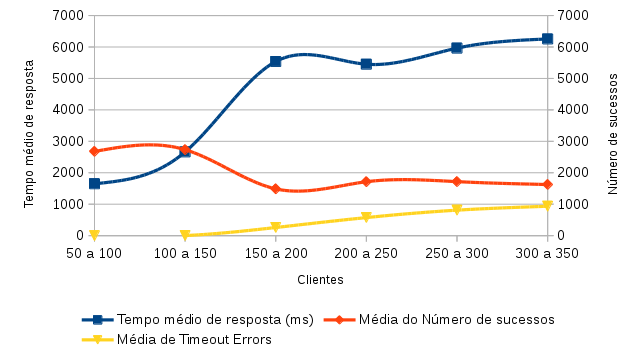
\includegraphics[width=.80\textwidth]{imagem/graficos/grafico_django_plano_de_teste_3_line.png}
    % Caption centralizada
    \captionsetup[grafico]{justification=centering}
    % Fonte
    \captionfont{\small{\textbf{\\Fonte: Dados da pesquisa}}}
    \label{grafico:teste-mantendo-carga-usuario-django-line}
  \end{grafico}
  
  Gráfico \ref{grafico:teste-mantendo-carga-usuario-django-line} correspondente ao plano de teste A-3, mantendo
  a carga de clientes, através do protótipo Django.
  
  \begin{grafico}[H]
    % Alterar espaçamentos antes e depois do caption
    \setlength{\abovecaptionskip}{5pt}
    \setlength{\belowcaptionskip}{0pt}

    % Caption
    \caption[Mantendo a carga de usuários no Node.Js por linha]
	    {Mantendo a carga de usuários no Node.Js por linha}
    \centering
    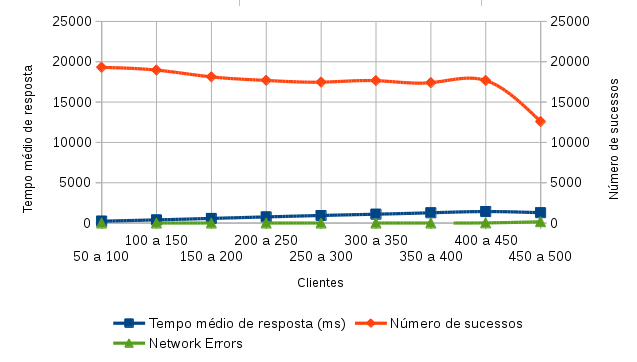
\includegraphics[width=.80\textwidth]{imagem/graficos/grafico_node_plano_de_teste_3_line.png}
    % Caption centralizada
    \captionsetup[grafico]{justification=centering}
    % Fonte
    \captionfont{\small{\textbf{\\Fonte: Dados da pesquisa}}}
    \label{grafico:teste-mantendo-carga-usuario-node-line}
  \end{grafico}
  
  Gráfico \ref{grafico:teste-mantendo-carga-usuario-node-line} correspondente ao plano de teste B-3, mantendo
  a carga de clientes, através do protótipo Node.Js.
  
  Nos gráficos \ref{grafico:teste-mantendo-carga-usuario-django-line} e \ref{grafico:teste-mantendo-carga-usuario-node-line}, que
  refere-se ao plano de teste A-3 e B-3,  pode-se interpretar com maior facilidade o desempenho do Node.js possuindo um maior
  número de sucessos e um aumento pequeno no tempo médio de resposta da aplicação. Enquanto no primeiro gráfico 
  \ref{grafico:teste-mantendo-carga-usuario-django-line} o primeiro gráfico o tempo de resposta aumentou devido a quantidade
  de usuários na fila do sistema e com isso uma queda abrupta na média de número de sucessos.
  
  Um dos fatores a serem considerados, foi no desenvolvimento da aplicação, pois com o \textit{framework} Django tem-se um rápido 
  desenvolvimento do software capaz de fornecer uma API robusta com poucas linhas de código. No \textit{framework} Express.Js o desenvolvimento
  é custoso para desenvolvedores menos experientes pois se trata de uma nova abordagem e paradigma. 
  O outro ponto a ser considerado é a maturidade do \textit{framework} Django, desde de 2005, e da linguagem Python. O Node.Js
  nasceu em 2009 e apesar de ter uma ampla comunidade \textit{open source} que contribui com código e bibliotecas complementares
  ao sistema ha muitas linhas de código a serem escritas. 
 
  
\section{Trabalhos futuros}
% Label para referenciar
\label{trabalhos-furutos}
  
  Este trabalho pode ser considerado um ponto de partida para conhecer a tecnologia e ambiente desenvolvimento de aplicativos 
  para Web, com foco no desempenho. Assim como as possibilidades de continuação e refinamentos deste trabalho 
  são variadas o Node.Js pode ser explorado em diversos outros contextos, tais como aplicações em tempo real, \textit{stream} de dados dentre 
  vários outros usos.
  
  No Brasil o Node.Js é pouco difundido e requer de mais estudos e materiais em língua portuguesa para os desenvolvedores iniciantes
  e empresas que desejam superar barreiras de escalabilidade com software. 
  
  Para refinar e explorar o ambiente do Node.Js, propõe-se aumentar a complexidade do protótipo utilizando como por
  exemplo, um serviço de \textit{upload} de arquivos ou até mesmo aumentar os recursos desta API REST para analisar 
  a deterioração do desempenho.
 
  Uma melhoria em nível do protótipo Django, objeto comparativo, seria a utilização de cache de consultas e dos resultados em \ac{JSON} que poderiam
  reduzir o tempo de resposta e aumentar o número de sucessos. Este cache pode ser colocado no \textit{framework} e utilizar também
  softwares \textit{memcached}\footnote[20]{Sistema de cache em memória distribuída. Disponível em http://memcached.org/} e/ou \textit{varnish}
  \footnote[21]{Acelerador de aplicativos Web. Disponível em https://www.varnish-cache.org/} em um outro servidor.\cite{usandodjango}
  
  Também é valido considerar a troca do \textit{framework} Django para o Tornado\footnote[22]{Web framework e biblioteca de rede 
  assíncrona. Disponível em http://www.tornadoweb.org/en/stable/} escrito em Python.
  Esta última tecnologia apresentada é um ótimo objeto de estudo e que poderia comparar as duas tecnologias, Node.Js e Python, pois 
  o Tornado possui características não bloqueantes e assíncronas.\cite{tornadogloboesporte}

  Após a implementação de todas essas funções ou até mesmo a troca de tecnologia do protótipo comparativo, 
  deverá ser executado novamente o plano de teste e o mesmo ambiente de teste para que não altere os resultados. Com estes
  resultados é possível identificar os impactos causados pelas modificações efetuadas no desenvolvimento do software.